\chapter{High Voltage System}
\label{ch:fddp-hv}

%%%%%%%%%%%%%%%%%%%%%%%%%%%%%%%%%%%%%%%%%%%%%%%%%%%%%%%%%%%%%%%%%%%%
\section{High Voltage System (HV) Overview}
\label{sec:fddp-hv-ov}


%%%%%%%%%%%%%%%%%%%%%%%%%%%%%%%%%
\subsection{Introduction}
\label{sec:fddp-hv-intro}

A \dword{lartpc} requires an equipotential cathode plane at high voltage and a precisely regulated interior electric field to drive 
electrons from particle interactions to sensor planes.  In the case of the DUNE \dlong{dp} technology, 
this requires a horizontal cathode plane, held at negative high voltage; a horizontal charge readout plane (CRP) in gas phase as described in  Chapter~\ref{sec:fddp-crp-intro}; and formed sets of conductors at graded voltages surrounding the
 the central drift volume, collectively called the \dlong{fc} as shown in Fig.~\ref{fig:dune_dp_fd}. The \dword{fc} consists of continuous field shaping rings that provide voltage degradation in vertical direction and forms a one contiguous active volume.


\begin{dunefigure}[A DP Overview]{fig:dune_dp_fd}
{A cutaway showing an overview of a DP detector module, showing the cathode plane and the photon detector on the floor and the 12m tall field cage modules surrounding the active volume, as well as the anode plane, the only part of the charge readout plane (CRP) visible in this angle}
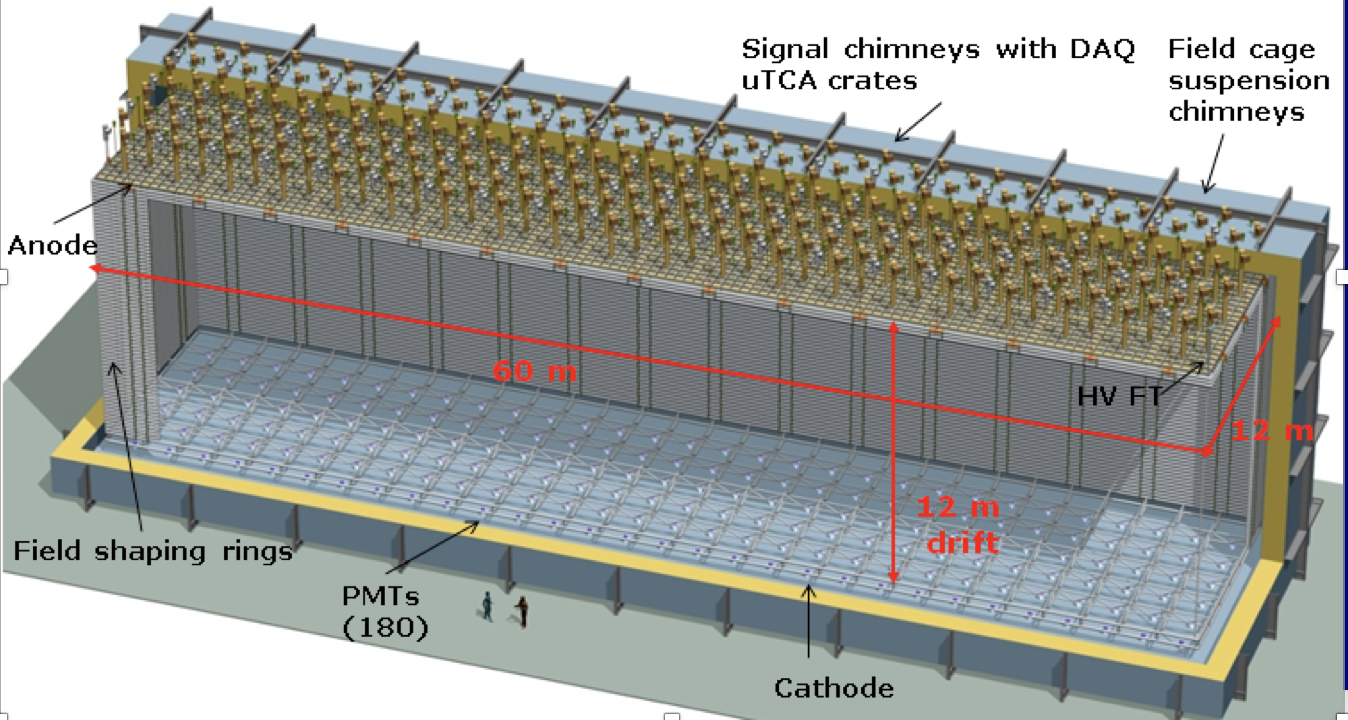
\includegraphics[width=0.8\textwidth]{Overview_Cutaway.png}
\end{dunefigure}


The \dword{hv} consortium provides systems that operate at the nominal voltages to provide the uniform $500V/cm$ electric field in the \dword{tpc} drift volume. As a result, its systems actually constitute a large fraction of the total internal structures of the \dword{tpc} itself. Mechanical and structural concerns are taken into account together with electrical design to meet the requirements. 

%%%%%%%%%%%%%%%%%%%%%%%%%%%%%%%%%%%%%
\subsection{Design Considerations}
\label{sec:fddp-hv-des-consid}


The \hv system is designed to meet the physics requirements of the DUNE experiment. This includes both physical requirements (e.g., an \efield 
that allows robust event reconstruction) and operational (e.g., 
avoidance of over-complication in order to maximize data collection efficiency). 
A collection of essential requirements for the high voltage system is shown in Table~\ref{tab:hvphysicsreqs}.

\begin{dunetable}
[\hv System Requirements]{p{0.05\textwidth}p{0.2\textwidth}p{0.35\textwidth}p{0.15\textwidth}p{0.15\textwidth}}
{tab:hvphysicsreqs}
{HV System Requirements}
No. & Requirement & Physics Requirement Driver & Requirement & Goal \\ \toprowrule
1 & Exceed minimum \efield TPC drift volume & Maintain adequate particle ID, which is impacted by slower drift speed and increased recombination, diffusion and space charge effects. & >\SI{250}{V/cm} &\SI{500}{V/cm} \\ \colhline
 2 & Do not exceed maximum \efield in \lar volume & Avoid damage to detector to enable data collection over long periods. & \SI{30}{kV/cm} & \dword{alara} \\  \colhline
3 & Minimize power supply ripple & Keep readout electronics free from external noise %, which confuses event reconstruction.  
\\ \colhline
4 &  Maximize power supply stability & Maintain the ability to reconstruct data taken over long period.  Maintain high operational uptime to maximize experimental statistics. \\ \colhline
5 & Provide adequate decay time constant for discharge of the cathode plane and \fc as well as cathode plane resistive segmentation & Avoid damage to detector to enable data collection over long periods. Maintain high operational uptime to maximize experimental statistics. & \si{\giga\ohm} resistors per each connection of the $3\times3$m$_2$ cathode units  \\ \colhline
6 & Provide redundancy in all \hv connections & Avoid single-point failures in detector that interrupt data taking. & > 2 voltage divider chains to distribute \hv to the \fc profiles & one voltage divider chain every four \fc modules\\ 
\end{dunetable}

%%%%%%%%%%%%%%%%%%%%%%%%%%%%%%%%
\subsection{Scope}
\label{sec:fddp-hv-scope}
The scope of the \hv system 
includes the continued procurement of materials for, and the fabrication, testing, delivery and installation of systems to generate, distribute, and regulate voltages so as to create a precision \efield within the \detmodule volume. 

The \hv system consists of components both exterior and interior to the cryostat. The \hv power supply is located external to the cryostat.  In DUNE DP FD, the \hv power supply is thought to be located on top of the \hv \fdth. HV is further distributed by interior components that form part of the TPC structure, as depicted in Figure~\ref{fig:dune-dp-hvs}.a.  These components are:


\begin{itemize}
\item power supply
\item \dword{hv} \fdth
\item \hv extender and voltage degrader
\item cathode plane \& ground plane
\item \fcage
\item \hv return \fdth and resister box
\end{itemize}


\begin{dunefigure}[HV system for a \dpmod ]
{fig:dune-dp-hvs}
{(a) A schematic overview of the \hv system for a \dpmod{}, 
(b) a photo of the \SI{300}{\kV} Heinzinger power supply\footnote{Heinzinger\texttrademark{} PNChp 300000 power supply.} used in the $3\times 1\times 1$ pilot \dual detector, (c) the VHV feedthrough used in the $3\times 1\times 1$ pilot \dual detector and (d) the \hv return connection used in the $3\times 1 \times 1$ pilot \dual detector}
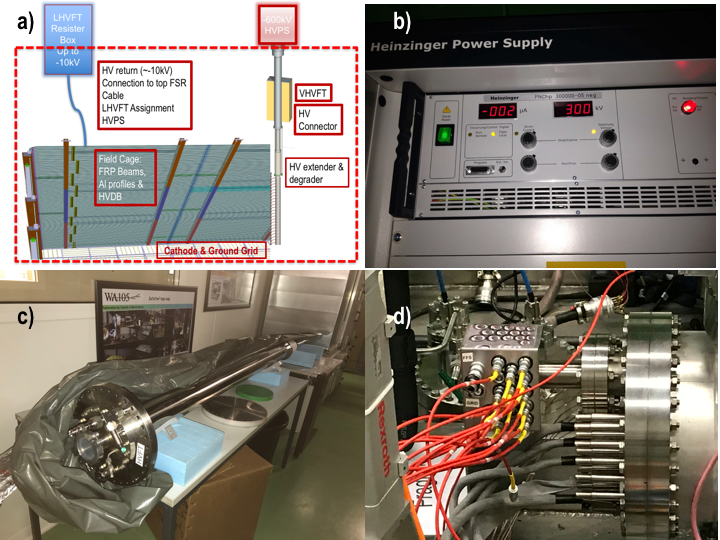
\includegraphics[width=1.0\textwidth,height=1.2\textwidth]{dp-hvs-n-photos.png}
\end{dunefigure}

%%%%%%%%%%%%%%%%%%%%%%%%%%%%%%%%
\subsection{System Overview}

A \dpmod  has a single modular cathode plane that forms the bottom of the single  \SI{12}{\m} (W) $\times$ \SI{12}{\m} (H) $\times$ \SI{60}{\m} (L) drift volume. It is constructed of eighty \SI{3}{\m} $\times$ \SI{3}{\m} contiguous units. 
The cathode units consist of stainless steel tube frames that hold a stainless steel grid. It is kept at a potential of \SI{-600}{\kV}.  A similar but highly transparent ground plane is placed just above photon detector system below the cathode to shield it from the high voltage.
The cathode bias is provided by an external \hv power supply through a \hv \fdth and a voltage extender unit that reaches the cathode.
 
The \fc surrounds the drift volume in a set of equidistant, stacked, horizontal, rectangular-shaped aluminum rings. Its function is to ensure a uniformity drift field of \SI{500}{\V\per\cm}. This is accomplished by gradually decreasing the voltage over the \SI{12}{\m} height from the cathode voltage of \SI{-600}{\kV} to \SI{-10}{\kV} at the top-most field shaping ring, to allow for the electron extraction into the gas volume of the \dword{crp}. The \fc consists of aluminum field-shaping rings, made up of mechanically and electrically connected $3m$ long aluminum profiles.  
This is a cost-effective system for establishing the required equipotential surfaces. 

%%%%%%%%%%%%%%%%%%%%%%%%%%%%%%%%%%%%%%%%%%%%%%%%%%%%%%%%%%%%%%%%%%%%
\section{HV System Design}
\label{sec:fddp-hv-design}

%%%%%%%%%%%%%%%%%%%%%%%%%%%%%%%%%%%%%%%%%
\subsection {High Voltage Power Supply and Feedthroughs}
The \dword{hv} delivery system consists of
\begin{itemize}
\item one power supply,
\item \hv cryogenic \fdth{}s,
\item an \hv cryogenic extender.
\end{itemize}

To ensure the nominal electric field of \SI{500}{V/cm} over  the \SI{12}{\m} drift distance, an external power supply shall be capable of delivering \SI{-600}{\kV} to  the cathode through one \hv cryogenic \fdth, with a maximum current draw of \SI{0.5}{\milli\ampere}.
At present such a power supply does not exist, but  Heinzinger, the industrial partner and leader in the production of \hv power supplies, is executing a vigorous R\&D program towards this goal, relying on the following facts:

\begin{itemize}
\item \SI{600}{\kV} power supplies are feasible, scaling the present industrial technology;
\item The same is possibly true for the \hv cryogenic \fdth, scaling to large diameter and longer size with respect to the present \SI{300}{\kV} prototypes;
\item The critical points of the \hv distribution are then the cable and its connectors on the power supply and on the \hv{}-\fdth. 
\end{itemize}

The joint R\&D program between DUNE and Heinzinger aims to eliminate cables and connectors, and build a power supply that can be plugged directly on the top of the \hv{}-\fdth.  A sample schematic and some details are shown in Figure~\ref{fig:dune-dp-hvps-ft}. 
Heinzinger is motivated to pursue this effort because of possible new industrial applications.

\begin{dunefigure}[HV PS and FT for a \dpmod ]
{fig:dune-dp-hvps-ft}
{(a) Vertical cross section of the proposed VHV power supply inserted over the 750 kV HVFT for a \dpmod{}, 
(b) Insertion detail of the proposed VHV power supply inserted over the 750 kV HVFT. The female HDPE of the HVFT is indicated in green. The male plug of the HVPS, shown inserted, is a metallic conductor inserted in a HDPE insulating tube (indicated in yellow. The gap between male and female is filled, via a tube inside the HVPS (not indicated) by silicone oil as RHODORSIL 47 V1000. (c) Vertical cross section of the HVPS. The front panel is on the left. The HV multiplication and regulation (not indicated) is in the beige region.}
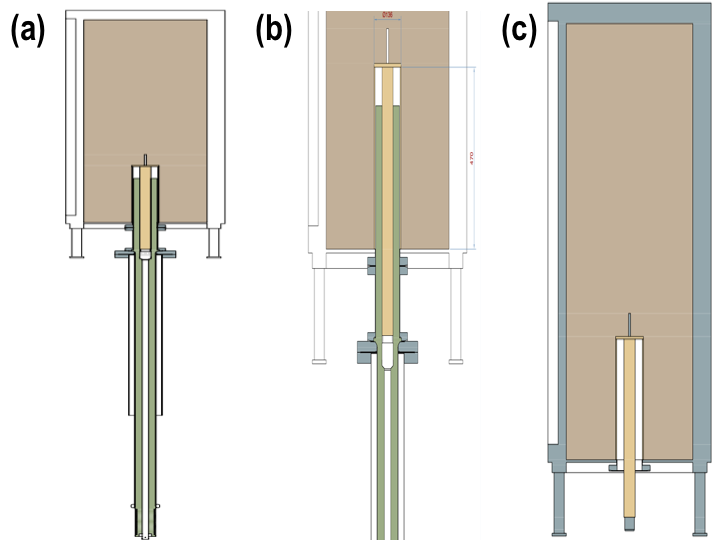
\includegraphics[width=0.5\textwidth]{dp-hvps-750kv.png}
\end{dunefigure}


Typical Heinzinger power supplies have ripples in the range of $\sim$\SI{30}{k\hertz} with an amplitude of $0.001\%V_{nom} \pm 50$ mV. Low-pass RC filter designed to reduce the voltage ripple could be integrated into the output of the power supply.  It, however, should be noted that the required ripple suppression does not need to be as high as for the \dword{spmod} thanks to the \dword{dpmod}'s more effective shielding of the anodic structure, performed by the extraction grid and by the CRP signal amplification stage. 

%Assuming the distance between the power supply and the cathode to be \SI{15}{\m} and the capacitance of the \fdth and \hv extender to be about \SI{100}{\pF/\m}, a resistance of a few M$\Omega$ integrated at the output of the power supply is sufficient for noise reduction.

The \hv \fdth is based on the same successful ICARUS design that was adopted in \dword{pdsp} and \dword{pddp}.  In this design, the voltage is transmitted by a stainless steel center conductor on the warm exterior of the cryostat, where this conductor mates with a cable end.  Inside the cryostat, the end of the center conductor has a spring-loaded tip that  contacts a receptacle cup mounted on the cathode, from which point \hv is delivered to the \fc.  The center conductor of the \fdth is surrounded by Ultra-High Molecular Weight Polyethylene (UHMW PE).  


To first order, the upper bound of operating voltage on a \fdth is set by the maximum \efield on the \fdth.  Increasing the insulator radius reduces the \efield.  For the target voltage, the \fdth uses a UHMW PE cylinder of at least \SI{15.2}{\cm} (\SI{6}\,in) diameter.  In the gas space and into at least \SI{15.2}{\cm} of the liquid, a tight-fitting stainless steel ground tube surrounds the insulator.  The ground tube has a Conflat flange of at least \SI{25.4}{\cm} (\SI{10}\,in) welded on for attachment to the cryostat.  A prototype\footnote{The prototype was manufactured by the company CINEL\texttrademark{} Strumenti Scientifici Srl.}  was successfully tested up to \SI{-300}{\kV} in pure argon in a dedicated setup; two similar prototypes are currently being installed in \dword{pdsp} and \dword{pddp}.


%%%%%%%%%%%%%%%%%%%%%%%%%%%%%%%%%%%%%%%%%
\subsection{High Voltage Extender and Voltage Degrader}

Since the \hv has to be guided from the top of the cryostat to the cathode (\SI{12}{\m} below the \dword{lar} surface), an extension of the \hv \fdth is required, as shown in Figure~\ref{fig:pd-hvft-extender}a, b and c. The extender contains an inner conductor at \SI{-600}{\kV} surrounded by an insulator. Since the extension runs the entire height of the drift volume, metallic rings (degrader rings) are installed on the periphery of the extension close to the field-shaping ring. Each degrader ring is electrically connected to the field shaping ring at the same height thus guaranteeing that the \efield in the \lar between the extender and the field cage remains at 0.


\begin{dunefigure}[DP HVFT and Extender]{fig:dp-hvft-extender}{Pictures of High Voltage \fdth and \dword{hv} extender-degrader; a) Overview of the \dword{hv} FT, \dword{hv} Extender and the degrader chain, b) Details of the top portion of the \dword{hv} extender and its connections to the field shaping rings, c) The detail of the \dword{hv} extender and degrader connection to the bottom part of the FC, including the connection to the cathode plane}
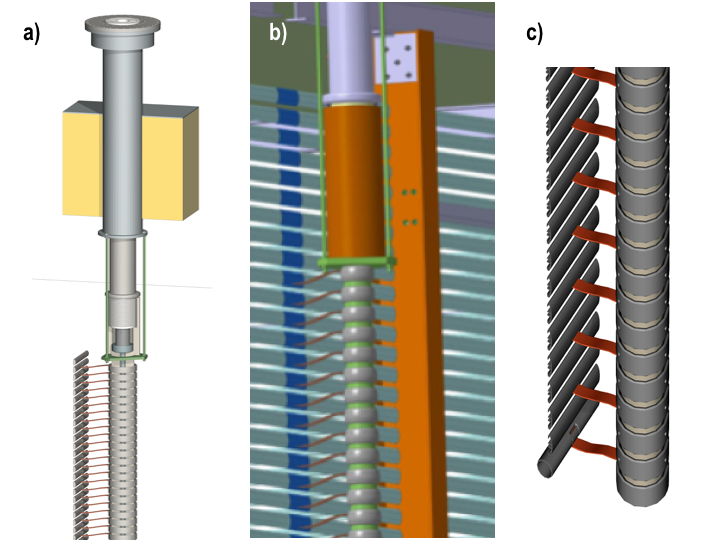
\includegraphics[width=0.75\textwidth]{dp-hvft-extender.png}
\end{dunefigure}

%%%%%%%%%%%%%%%%%%%%%%%%%%%%%%%%%%%%%%%%%
\subsection{Cathode Plane}

The \dpmod{}'s cathode plane forms the  bottom of the single  \SI{12}{\m} (W) $\times$ \SI{12}{\m} (H) $\times$ \SI{60}{\m} (L) drift volume and provides a constant potential surface at \SI{-600}{\kV}.  It receives its \hv from the central conductor of the extender that carries the voltage from the power supply through the \hv \fdth.  

The cathode plane consists of eighty \SI{3}{\m} $\times$ \SI{3}{\m} modules. 
The cathode module design is based on the design used in  \dword{pddp}, for which the cathode consists of a stainless steel (316L) mechanical structure made from
tubes of various diameters: an external frame made from \SI{60}{\milli\m} diameter tubes, internal oval pipes of $20mm\times 40mm$ with 1.5mm thickness, as shown in Fig.~\ref{fig:dune-dp-cathode}. 
This frame is filled with smaller tubes of \SI{12}{\milli\m} diameter (not shown in the figure), forming a grid, to provide uniformity of the quippotential surface, while ensuring 60\% optical transparency. All diameters were optimized to guarantee a uniform potential  potential across cathode and to satisfy the maximum local field requirement of $30kV/cm$ minimize the local \efield{}s to ground.
The cathode plane consists are bolted together and fixed to the supporting FRP I-beams of the \fc. 


\begin{dunefigure}[Cutaway view of \dword{pddp} Cathode]{fig:dune-dp-cathode}
{A cutaway view of \dword{pddp} cathode(Credit: A. Gendotti)}
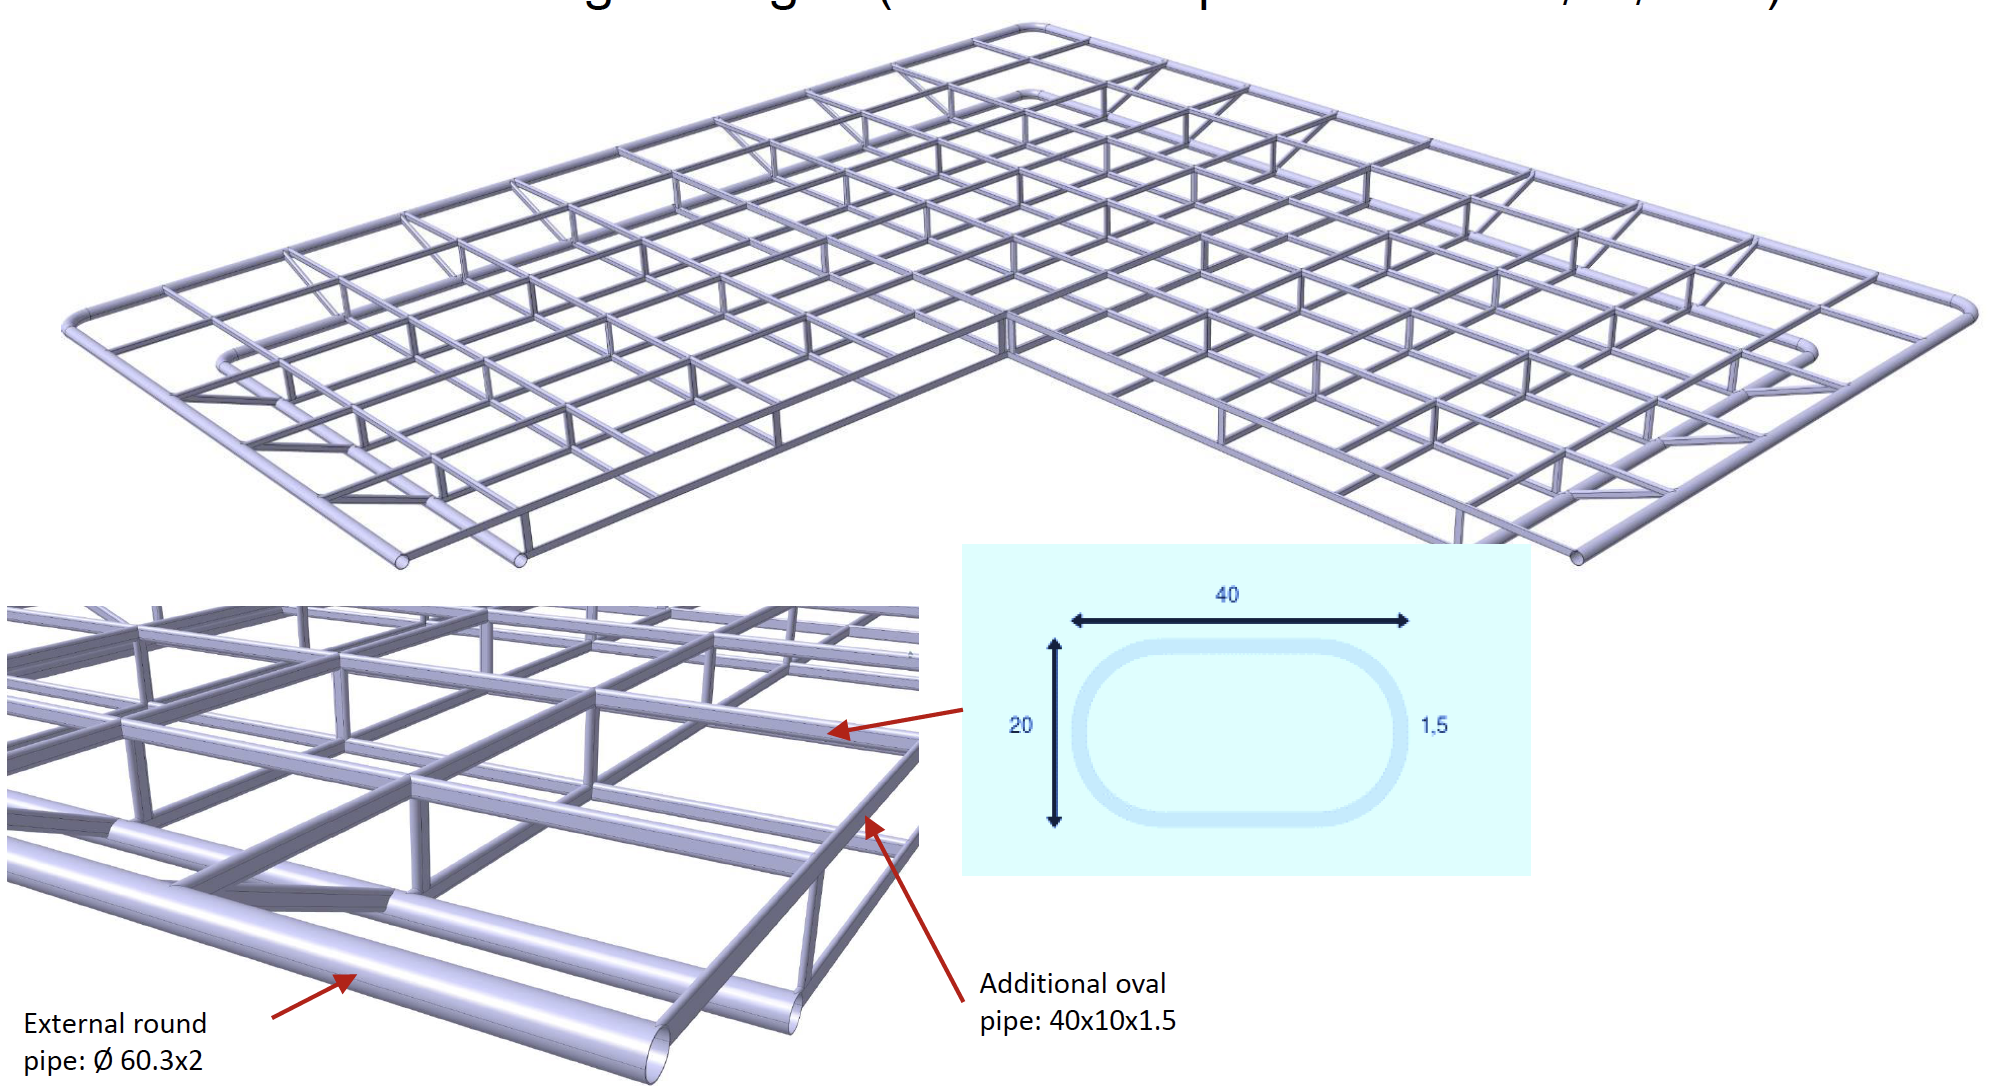
\includegraphics[width=0.8\textwidth]{dp-cathode.png}
\end{dunefigure}

\begin{dunefigure}[\dword{pddp} Cathode field]{fig:dune-dp-cathode-field}
{Place holder for field between cathode and the ground grid} 
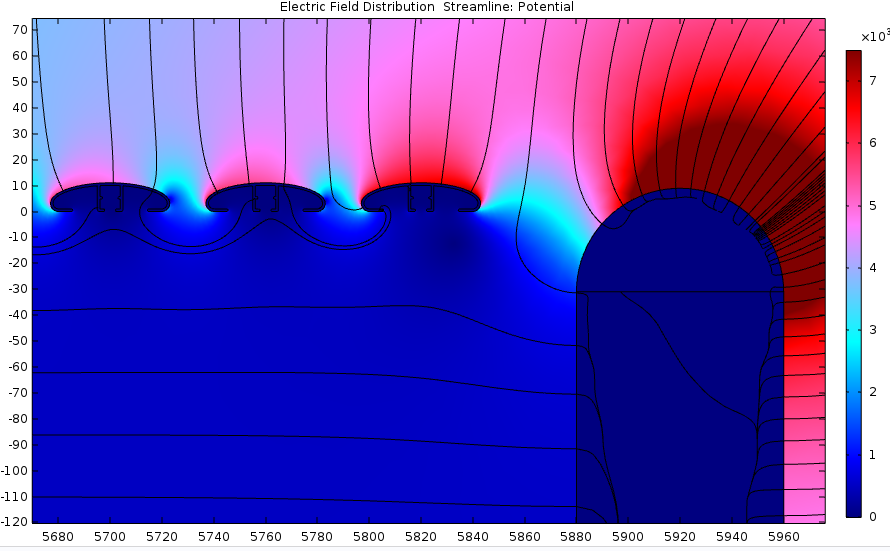
\includegraphics[width=0.7\textwidth]{field10.png}
\end{dunefigure}

The energy stored in the volume between the cathode plane and the ground grid (which sits under the cathode and above the \dwords{pd}) is estimated to be about \SI{1.7}{\kilo\joule} over the \SI{12}{\m} $\times$ \SI{60}{\m} area, based on the cathode voltage and the distance of \SI{1}{\m} between the cathode and the ground grid describe in the next section. 
A sudden discharge from the cathode frame to the cryostat membrane could cause severe damage to it.  The modular construction of the cathode helps minimize this effect in case of discharge. During assembly in the cryostat, the cathode units will be kept electrically insulated and connected to their adjacent neighbors through \si{\giga\ohm}  
resistors. Given the \SI{100}{\pico\farad} capacitance of each cathode unit, any discharge occurring in one unit will release at most 
\SI{21}{\joule} of stored energy while the discharge rate  
to the other units will be slowed down to the several hundred millisecond range.

Detailed calculations are in progress to determine the final shape and the size of the cathode and ground grid frames to meet the requirement that limits the maximum \efield to \SI{30}{\kV\per\cm}  
throughout the \lar volume (Fig.~\ref{fig:dune-dp-cathode-field}).  Structural calculations are also needed to verify the planarity of the cathode as it hangs on the \fc supports.
Value and voltage characteristics of the connecting resistors will also be defined according to results from dedicated simulations of the cathode electrical model.


%%%%%%%%%%%%%%%%%%%%%%%%%%%%%%%%%%%%%%%%%
\subsection{Ground Grid}
The ground grid is installed between the \dword{pd} and the cathode plane to shield the \pmt{}s from a discharge.  
%Similarly to the cathode, the ground grid consists of 316 L stainless tubes in \dword{pddp}. It also comes in 4 modules of dimension $3m\times 3m$ and is placed on the membrane floor by supporting feet. The central feet is glued to the membrane (STYCAST 2850FT). The ground for DUNE DP FD will use the similar structure, taking into account the field generated by the 600kV potential as in the case of the cathode.

The ground grid consists of 316 L stainless tubes, as does the cathode, and is made of eighty \SI{3}{\m} $\times$ \SI{3}{\m} modules. Unlike the cathode, the ground grid has a single layer supported a set of feet resting on the membrane floor.
Detailed studies on the grid geometry to ensure that the requirement on the maximum local field is satisfied.

%%%%%%%%%%%%%%%%%%%%%%%%%%%%%%%%%%%%%%%%%
\subsection{Field Cage}

\subsubsection{Mechanical Structure}
The field shaping rings of the \fc are made up of extruded roll-formed aluminum open profiles.  
The profiles are stacked horizontally and constructed into continuous rectangular rings that form the vertical sides of the drift volume. The aluminum profiles are attached to structural elements made of pultruded fiber-reinforced plastic (FRP). 


FRP is non-conductive and strong enough to withstand the \fc loads in the temperature range of \num{-150}\,C and \num{23}\,C.
This material meets the  Class A International Building Code classification for flame spread and smoke development, 
as characterized by ASTM E84. \fixme{is ASTM E84 a particular code?}  


Each of these modules is composed of three 
styles of submodules of dimensions \SI{3}{\m} (W) $\times$ \SI{2}{\m} (H). These submodules are supported by two \num{6}\,in FRP I-beams (with profile slots cut out) and two \num{3}\,in "cross bar" I-beams that form a rectangular frame.  


The \fc is modular, each module covering a vertical area of \SI{3}{\m} (W) $\times$ \SI{12}{\m} (H). 
There are two types of modules, straight section and corner, both types having the dimensions \SI{3}{\m} (W) $\times$ \SI{12}{\m} (H). A total of 72 straight section modules (i.e., with straight profiles) and eight corner section modules, with profiles bent \num{45} degrees at one corner to allow straight connections via clips at the corner as shown in Fig.~\ref{fig:dune-dp-fc-all}.c.  A photo of \dword{pddp} \fc is shown in Fig.~\ref{fig:dune-dp-fc-all}.d.

\begin{dunefigure}[DP FC Parts]{fig:dune-dp-fc-all}
{Field Cage Parts and connections for \dword{pddp} detector.  a. One \dword{pddp} FC Panel which consists of three sub-modules.  DUNE DP has virtually identical structure, except for the number of middle sub-module to be four, b. A photo of the top module connection to the stainless steel I-beam and an inter-submodule connection, c. Aluminum clip connection at the corner and at straight sections, d. \dword{hv} Divider Board and their connections on \dword{pddp} \fc }
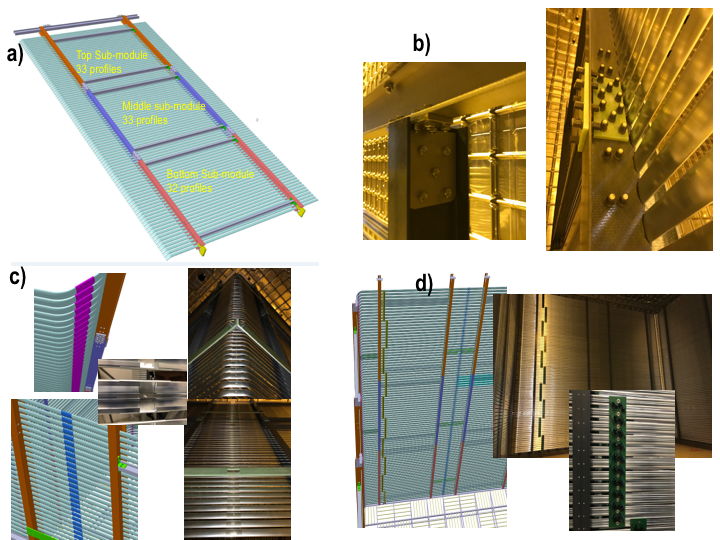
\includegraphics[width=1.0\textwidth,height=1.0\textwidth]{dp-fc-parts.png}
\end{dunefigure}


Each \fc module is made of six submodules of three distinct types: top, bottom and middle. The dimensions for all submodules are \SI{3}{\m} (W) $\times$ \SI{2}{\m} (H).
Each module has one top submodule with 33 profiles, four middle submodules with 33 profiles each, and one bottom submodule with 32 profiles, for a total of 197 profiles per module. The voltage of the top-most field shaping ring  is \SI{-9}{\kV}. 
The top submodules make the mechanical connection to the ceiling of the cryostat from which the entire \fc hangs as shown in Fig.~\ref{fig:dp-fc-installation-connection} left ; the bottom modules make both mechanical and electrical connections to the cathode. 


A railed rib runs along the length of the aluminum profiles at the center of the profile.  The rib provides mechanical strength and acts as the rail for the slip nuts that hold the profiles onto the supporting fiber reinforced plastic (FRP) frame. The rib also serves as the rail for the nuts that hold the \hv divider boards and the slip nuts for inter-module profile connections.  
All profiles at a given height are electrically connected via an aluminum clip screwed onto the slip nut across two neighboring profiles.  A resistive divider chain interconnects the aluminum profiles to provide a linear voltage gradient between the cathode and the top field-shaping ring.   


The extruded aluminum profiles are mounted to the \SI{15.2}{\cm} (\num{6}\,in) I-beam via two stainless screws and aluminum slip nuts in the center enforcement rail of the profile only on one of the \SI{15.2}{\cm} I-beams to allow contraction on either side of the profile. The top submodule has an extended \SI{15.2}{\cm} FRP beam with holes to connect it to the stainless steel I-beam hanging from the ceiling.  The bottom submodule has a cut-out to hold the cathode plane onto it. The four middle submodules are symmetric and thus are interchangeable.


\subsubsection{Electrical Interconnections}

An aluminum clip connects the ends of each set of two end-to-end \fc profiles, forming continuous equipotential rectangular rings  \SI{144}{\m} long. 
 \Dword{hv} divider boards (HVDB), consisting of two resistors and a series of four surge protection varistors in parallel, bridge the gap between the two neighboring stacked profile rings.   The total number of rows of HVDB will be determined based on the redundancy and the current limit requirements;  one row of HVDB is in principle sufficient to provide the required potential difference of \SI{3}{\kV} between neighboring rings, but more is desirable for redundancy.


The resistive chain for voltage division between the profiles provides a linear voltage gradient between the cathode and the top-most field shaping ring. It is critical as it determines the strength of the \efield between one profile and its neighbors, as well as between the profile and other surrounding parts, e.g., the grounded stainless steel membrane. The \efield needs to be kept well below \SI{30}{\kV\per\cm} at all points in the \lar bath to enable safe TPC operation.

The identified profile, Dahlstrom Roll Form \#1071,
\footnote{Dahlstrom Roll Form \#1071, Dahlstrom\texttrademark{}.}  is estimated to lead to \efield{}s of up to \SI{12}{\kV\per\cm}  
for the planned \fc configuration and operating voltage. Figure~\ref{fig:profile-e-field} illustrates results from an \efield calculation.


\begin{dunefigure}
[Electric field map and equipotential contours of an array of roll-formed profiles]{fig:profile-e-field}
{Electric field map (color) and equipotential contours of an array of roll formed profiles biased up to \SI{-300}{\kV} and a ground clearance of about \SI{100}{\cm} in \dword{pddp}(CAD model)} 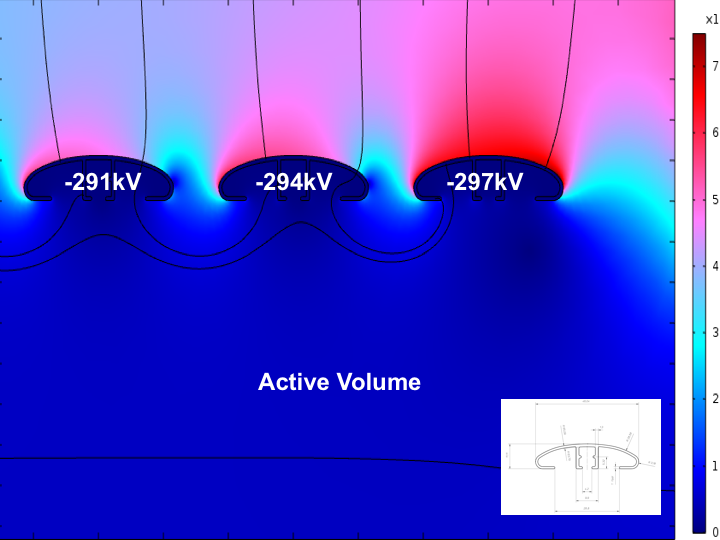
\includegraphics[width=0.8\textwidth]{pddp-field-map.png}
\end{dunefigure}

Two distinct types of \hv divider boards are used for \dword{pddp} - 10 stage and 8 stage boards.  Each stage consists of two 2 $G\Omega$ resistors in parallel and four variable resistors of threshold voltage 1.28kV to protect the resisters in case of a sudden discharge.  The total expected current at 600kV therefore is 3 $\mu A$ per row.  Since multiple rows which are connected in parallel will be used for redundancy, the expected current in the entire system is simply number of rows times the current per each row.
For optimization purposes, one DUNE DP HVDB will connect 11 stages.  This enables to cover one $12m$ tall module to be covered by fifteen 11 stage HVDB and one 10 stage HVDB at the bottom to make the final connection.  


Figure~\ref{fig:dp-hvdb} shows one HVDB board and  Fig.~\ref{fig:dune-dp-fc-all}.d. show the connection of one row of HVDB through the entire height of the \fc as installed in the \dword{pddp}. The  \SI{12}{\m} (W) $\times$ \SI{60}{\m} (L) ground plane consists of 80 unit planes (each \SI{3}{\m} $\times$ \SI{3}{\m}).  
The cathode plane is mounted to the bottom of the \fc, together forming one contiguous unit of field-providing structure.  The bottom-most HVDB makes the connection between the cathode and the bottom-most field-shaping ring.
For redundancy, a total of two HVDB rows are used in \dword{pddp}.  
The \dpmod will use one HVDB chain every four \fc modules, providing an ample redundancy.  However, the final number of rows of HVDB must take into account the impact of the underlying current through the \fc to the particle interactions.


\begin{dunefigure}[DP HVDB]{fig:dp-hvdb}{\dword{pddp} high voltage divider board a) schematic circuit diagram, b)photo of the top of the board, c) photo of the bottom of the board}
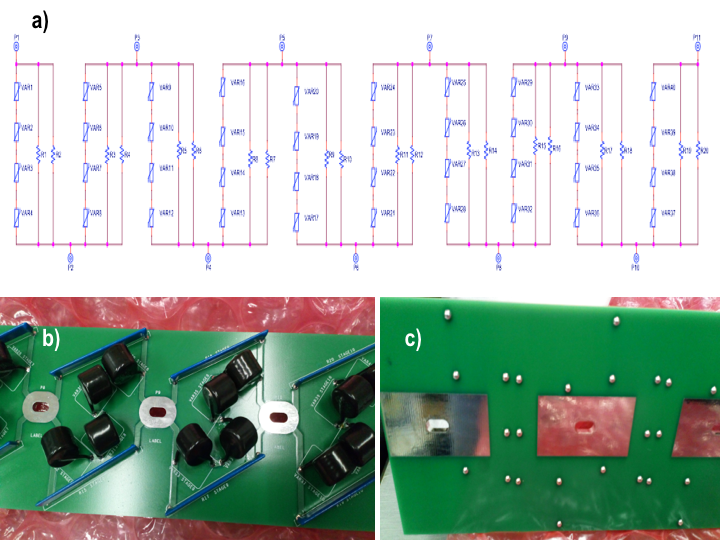
\includegraphics[width=0.75\textwidth]{dp-hvdb.png}
\end{dunefigure}


\begin{dunefigure}[DP field cage installation process and intermodule connection]{fig:dp-fc-installation-connection}{Left: Two sub-modules connected and hanging from the two sets of stainless steel cables from the ceiling.  The lifting wires are used to raise the module to its position as sub-modules are connected and the hanging wires keep the fully integrated module into its final position.  Right: These show inter-sub-module connections.  Each connection is made by two 1cm thick G10 plates along the height of the I-beams and one 1cm thick G10 plate on the flange.}
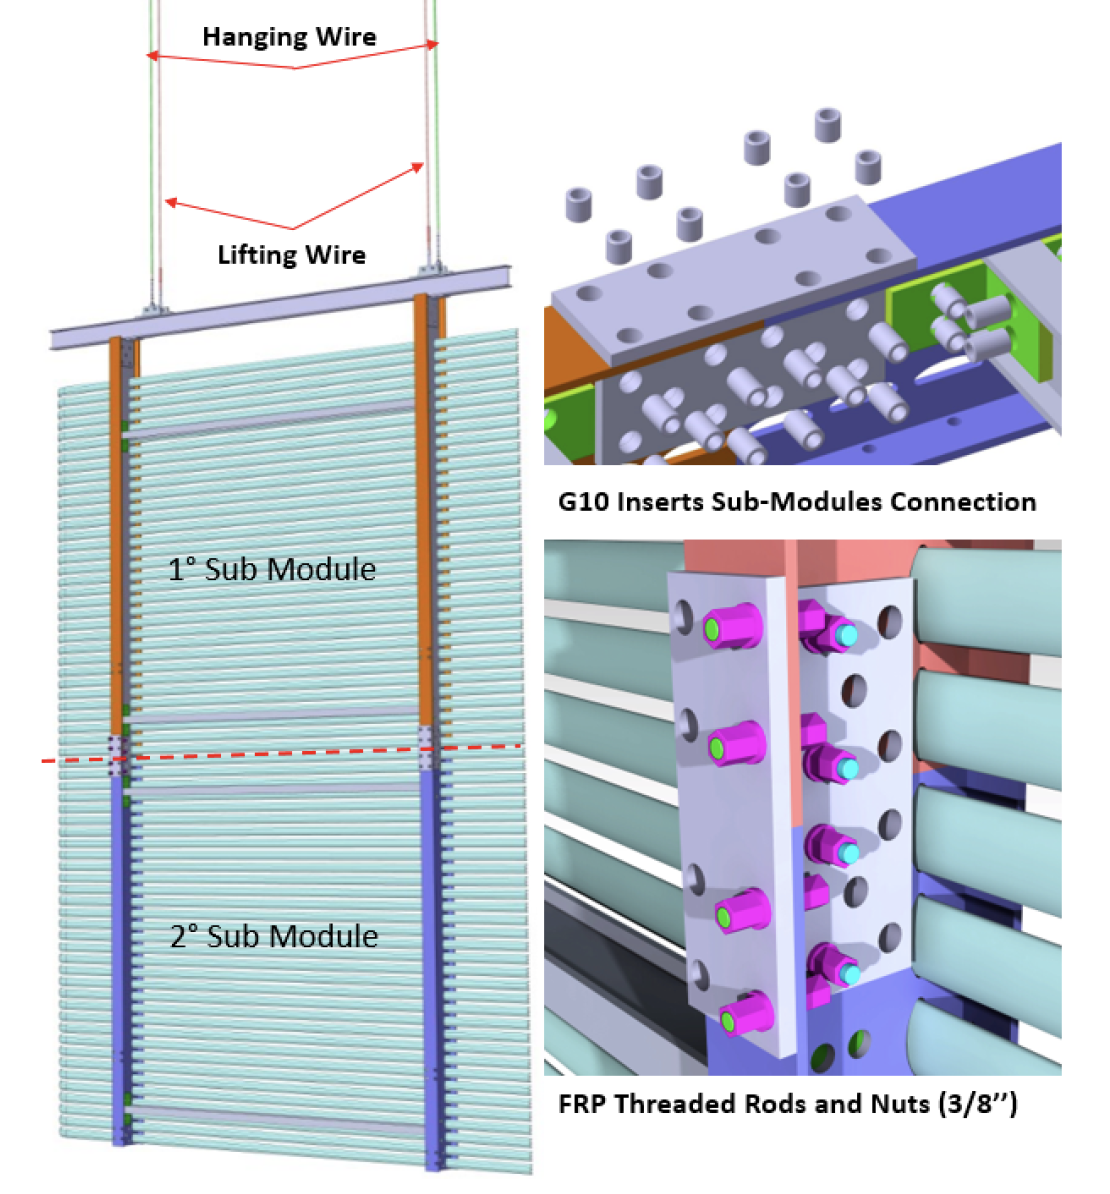
\includegraphics[width=0.75\textwidth]{module-connection-installation.png}
\end{dunefigure}


%%%%%%%%%%%%%%%%%%%%%%%%%%%%%%%%%%%%%%%%%
\subsection{HV Return and Monitoring Devices}

In order to maintain the potential difference between the top most field shaping ring and the extraction grid of the charge readout plane, either a dedicated separate high voltage supply and an adjustable resistor chain is used in the HV return outside of the cryostat.  This requires an independent 10kV feedthrough similar to those developed for the extraction grid.

Multiple devices are planned for monitoring the \hv.  
\begin{itemize}
\item The Heinzinger units have typical sensitivities down to tens of nanoamperes with current readback capability.  The units are able to sample the current and voltage every few \SI{100}{\milli\s}.  
\item Inside the cryostat, so-called pick-off points near the anode will monitor the current through the HVDB resistor chain.  

Additional pick-off points could be implemented on the ground grid below the cathode to monitor the possible stray currents.
\end{itemize}
\noindent 


%%%%%%%%%%%%%%%%%%%%%%%%%%%%%%%%%%%%%%%%%%%%%%%%%%%%%%%%%%%%
\section{Quality Assurance}
\label{sec:fddp-hv-qa}

{\bf Field Cage FRP Parts} Upon delivery of the FRP I-beams and other parts, all parts will undergo a visual inspection process to look for defects, in particular those affecting structural integrity, such as cracks, air bubble holes, depression and flatness. The parts will be sorted into three preliminary categories: category 0 (pass), category 1 (problematic but could be repairable) and category 2 (severe and unusable) .

The visual inspection will be followed by critical dimension measurements to verify individual submodule assembly and module interconnection integrity.  These measurements will focus on cross sectional dimensions for rods, plates and bars, and on the length, straightness, flatness and camber of the beams and flanges.
All measurements must satisfy the mechanical tolerance provided by the design drawings and the standard industry quality criteria.

The FRP I-beams and parts in category 1 will undergo a repair process during the preparation stage through defibering, deburring and sanding.  Another set of measurements will be performed after the repair to determine the category of the repaired part.

Those in category 2 will be returned to the vendor for replacements.

{\bf High Voltage Divider Board}
All resisters used for board production are numbered and undergo three step quality testing for final selection; 1. room temperature resistance measurement at voltages up to 4kV in 500V steps, 2. liquid nitrogen resistance measurement at voltages up to 4kV in 500V steps and 3. resistance measurement at voltages up to 4kV in 500V steps after warming up to room temperature.  Once the resistance of all resistors are measured, the measured resistance values are histogrammed for the final selection.   The selection is made based on the grouping of the resistors whose resistance are within 1\$ of each other using the results from all three testing stages.   Since it is more important to have the resistance values close to each other than being the given value, unless they are totally out of range from the design values, selecting the tighter grouping provide better quality assurance.  

All varistors for board production are also numbered for quality assurance and undergo three step quality testing for the final selection; 1. room temperature clamping voltage measurement, 2. liquid nitrogen clamping voltage measurement and 3. clamping voltage measurement after warming up to room temperature.  Once the clamping voltages of all varistors are measured, the measured clamping voltages in all thee stages are histogrammed separately for the final selection.   The selection is made based on the clamping voltage closer to the design values to ensure proper protection.   

Once the electrical parts are mounted on the HVDB by the vendor, they undergo three step quality assurance tests; 1. room temperature resistance measurement of each stage, 2. liquid nitrogen resistance measurement of each stage and 3. resistance measurement of each stage after warming up to room temperature.  These measurements for each board is histogrammed and used for HVDB selection.  The boards with any of the resistance of any stage is more than 0.5\% out of the mean do not pass the quality assurance.  The boards are in three categories: 0. Pass, 1. Repairable and 2. Reject.  Board in category 1 will be sent back to the vendor with the selected resisters so that the parts in the failed stages can be replaced.

{\bf Aluminum Profiles and Clips}
The quality of aluminum profiles and clips will be done on prototype production samples prior to the full production.   The samples will be visually inspected for the shape and the adherence to the design drawing, the smoothness of the surface, the surface coating quality and the smoothness of the bend for the 45 degree bent profiles.  Clip samples will be visually inspected for the shape and the adherence to the drawing, the smoothness of the edges and the mechanical fitness and tightness to the profiles.


{\bf Cathode, HVFT and the Extender} The QA for other components are under development within the \dword{pddp} construction efforts.


{\bf Power Supply and Feedthrough} The power supply is tested extensively along with the controls and monitoring software.  Features to be included in the software are:
\begin{itemize}
\item Capability to ramp and change the voltage; rate change and pause capabilities and settings included. 
\item Capability to accept user-defined current limit.  This parameter sets the value of current at which the supply reduces the voltage output in order to stay below it.  The current limiting itself is done in hardware.
\item Capability to accept a setting for trip threshold current.  At this threshold the software would reduce the voltage output. 
In previous experiments, the trip function in software would set the output to \SI{0}{kV}. 
\item The software shall record the current and voltage readback values with a user-defined frequency, and also any irregular current or voltage events. 
\end{itemize}


\section{Production and Assembly}
\label{sec:fddp-hv-prod-assy}

%%%%%%%%%%%%%%%%%%%%%%%%%%%%%%%%%%
\subsection{Field Cage Submodule Frames}
\label{sec:fddp-hv-prod-assy-fc-frames}

%All FRP parts which passed the QC/QA process above will undergo the preparation process.  Each of the parts will be defibered, deburred, sanded to smooth the edge and varnished to further suppress remaining fibers.  Once the part completes the preparation process, they will be stored a humidity and temperature controlled drying area for 24 - 48 hours to fully cure the varnish.  Upon full curing of the varnish, each module will be laser engraved with a unique part number for quality data base recording.

%Once the FRP parts are prepared, the sub-module will be pre-assembled on the table prior to packaging to ensure fitness of all parts, including inserts, screws and slip nuts.   When the fitness is verified, the sub-module will be dissembled and packaged into a $20cm\times 20cm\times 2m$ compact package with edges will be wrapped with a thick plastic layer to protect the FRP parts from mechanical damage from a fall.  This package will include all necessary parts for the given sub-module assembly along with 10 - 20\% spare parts.  This ensures each package is self-sufficient for the final assembly.  Each package will be given a sub-module number for further tracking purposes.

%Many of these packages can be shipped to SURF underground for the final assembly prior to the installation.   The 3m long aluminum profiles will be produced separately and shipped to SURF as well for the final assembly.  The quality control of the profiles will be conducted as the sub-module is assembled.   Profiles with deep scratches and sharp protrusion that could provide excess charge concentration will be rejected.

%The final assembly of these sub-modules will be carried out inside the cryostat.   An assembly table with precision alignment bar for rapid profile alignment will be used for the assembly.   The package will be cut open on the table and the FRP frame which consists of two 6 inch I-beams and two 3 inch I-beam cross bars will be assembled with four L-brackets and sixteen 2.21 inch threaded rods through the G10 insert and eight 2.27 inch threaded rods through G10 inserts held by the plastic nuts.  These nuts will be hand-tightened first and then torque set using the specific setting (12V Dewalt Power Screw Driver torque set at 8).

%Once the FRP frame is put together, aluminum profiles will be inserted through the corresponding slots on the 6 inches beams either side.  One slip-nut for profile mounting needs to be inserted onto the center rib rail prior to the profile insertion into the FRP frame.  Care must be taken to ensure the profiles are not scratched during the insertion process. 

%Once all profiles are inserted, each of the profiles will be mounted onto the I-beam using two M4 button head- hex drive stainless steel screws with the length 5cm (check the number) onto the aluminum slip nut.   When all screws are hand tightened as much as possible, final torque setting will be applied using the 12V Dewalt Power Screw Driver torque set at 1.  The final alignment of the profiles will then be made using hand screwed driver only by tightening further one of the two screws.  A wheel based with a unistruct bars will then be mounted to the bottom of the sub-module and stored into an area for installation.   The wheel will have the sub-module number clearly attached for tracking purposes.


All FRP parts that pass the QA process undergo the preparation process, which involves \dword{qc} at each step.  Each of the parts is first defibered, deburred, sanded to smooth the edges, then varnished to
suppress any remaining fibers.  Once the part completes the preparation process, it is stored in a humidity- and temperature-controlled drying area for \numrange{24}{48} hours to fully cure the varnish.  Upon full curing, each module is laser-engraved with a unique part number and recorded in a QC database. 

At this point the submodule is pre-assembled on a table prior to packaging to ensure fitness of all parts, including inserts, screws and slip nuts.   When the fitness is verified, the submodule is disassembled and packaged into a \SI{2}{\cm}$\times$\SI{20}{\cm}$\times$\SI{2}{\m} compact package with the edges wrapped with a thick plastic layer to protect the parts from mechanical damage, e.g., from a fall.  This package includes all necessary parts to assemble the given submodule 
along with \numrange{10}{20}\% spare parts.  This ensures that each package is self-sufficient for the final assembly.  Each package is given a submodule number for further tracking purposes.  This sub-module number stays with it throughout the assembly at SURF and the final installation so that the given sub-module can be assigned to a specific module in the specific location within the module. 

These packages will be shipped to SURF underground 
for the final assembly prior to the installation.   
The \SI{3}{\m} long aluminum profiles are produced and shipped to SURF separately for final assembly.  The final QC of the profiles will be conducted during submodule assembly.   Profiles with deep scratches and sharp protrusions that could provide excess charge concentration will be rejected. This process must be done underground at the time of sub-module assembly since the delicate nature of the coated surface and the requirement of the smoothness to meet the local maximum field requirement.

The assembly of submodules from the parts will be carried out inside the cryostat.   An assembly table with a precision alignment bar for rapid profile alignment is used for the assembly.   The package is opened on the table and the FRP frame is assembled with four L-brackets and sixteen \SI{5.61}{\cm} (\num{2.21}\,in) threaded rods through the G10 insert and eight \SI{5.77}{\cm} (\num{2.27}\,in) threaded rods through G10 inserts held by the plastic nuts.  These nuts are hand-tightened first and then torque set using the specific setting (12V Dewalt Power Screw Driver\footnote{12V Dewalt\texttrademark{} Power Screw Driver \url{https://www.dewalt.com/} .} torque set at 8).

Once the frame is assembled, aluminum profiles are inserted through the corresponding slots on the \SI{15.2}{\cm} (\num{6}\,in) on either side.  One slip-nut 
is inserted onto the center rib rail prior to the profile insertion.  
Care must be taken to ensure the profiles are not scratched during the insertion process. 

Once all profiles are inserted into the frame, each of the profiles is mounted onto the I-beam using two \SI{45}{\mm} M4 button head hex drive stainless steel screws into the aluminum slip nut. 
When all screws are hand-tightened as much as possible, the final torque is applied using the 12V Dewalt Power Screw Driver torque set at 1.  The final alignment of the profiles is then made by hand, tightening only one or two screws, as necessary.
A wheel base made of unistrut bars is then mounted to the bottom of the submodule and the entire unit is placed in a designated area to await installation.   The wheel is clearly labeled with the submodule number for tracking purposes for installation.


%%%%%%%%%%%%%%%%%%%%%%%%%%%%%%%%%
\subsection{Cathode Plane}
\label{sec:fddp-hv-prod-assy-cathode}

%The \dpmod has one cathode plane that consists of multiple $3m\times 3m$ units to cover $12m (W) \times 60m (L)$, with one drift volume of $12m(W)\times 12m (H)\times 60m(L)$. There are eighty $3m\times 3m$ cathode units, installed contiguously at the bottom of the TPC. One $3m\times 3m$ cathode unit is made of stainless steel tube frame holding stainless steel grid.


Each cathode module is assembled off-site and shipped to SURF in its transport container.   The containers are transported underground to the cryostat and opened in front of the cryostat.  The cathode module is then inserted into the cryostat for installation.  The detailed installation process is under development in \dword{pddp}.

%%%%%%%%%%%%%%%%%%%%%%%%%%%%%%%%%
\subsection{Ground Plane} % Grid}
\label{sec:fddp-prod-assy-ground-grid}

%Ground Grid is placed at the membrane with nine Pillars. Center pillar will be point glued at the membrane in order to stay xed. The other eight external Pillar have a Te on sheet on their bottom in order to shrink freely during the cool down without inducing stress at the membrane

Each ground grid module is assembled off-site and shipped to SURF in its transport container.   The containers are transported underground to the cryostat and opened in front of the cryostat.  The ground grid module is then inserted into the cryostat for installation. The detailed installation process is under development in \dword{pddp}.


%%%%%%%%%%%%%%%%%%%%%%%%%%%%%%%%%
\subsection{Electrical Interconnections}
\label{sec:fddp-prod-assy-elec-connec}

The HVDB will be mounted on the profiles as the sub-modules are built.  For optimization purposes, one DUNE DP HVDB will connect 11 stages.  This enables to cover one $12m$ tall module to be covered by fifteen 11 stage HVDB and one 10 stage HVDB at the bottom to make the final connection.   One row of HVDB will be mounted every four \fc modules.  All connections and electrical functionality must be checked with high sensitivity electrometer.


%%%%%%%%%%%%%%%%%%%%%%%%%%%%%%%%%%%%%%%%%%%%%%%%%%%%%%%%%%%%%%%%%%%%
\section{Interfaces to the HV System}
\label{sec:fddp-hv-intfc}

%%%%%%%%%%%%%%%%%%%%%%%%%%%%%%%%%
\subsection{System to Cryostat}
\label{sec:fddp-hv-intfc-to-cryostat}

Each \fc module is suspended and raised by two ropes hung from the cryostat roof through the \fc suspension \fdth{}s, by winches as in \dword{pddp}.  

Once an \fc module of the full height is completed for \dword{dpmod}, it will be hung 
from the cables attached to the final suspension hook and the  
 the suspension \fdth is then fully sealed. 
A possible improvement on the \dword{pddp} interface is to use remote-controlled electrical wrenches (as opposed to manual) to ensure synchronized lifting of the modules.

%%%%%%%%%%%%%%%%%%%%%%%%%%%%%%%%%
\subsection{System to Charge Readout Plane}
\label{sec:fddp-hv-intfc-to-crp}

There shall be no direct hardware interface between the \hv and \dword{crp} systems. The cryostat penetrations and \fdth{}s for the two systems are completely independent, as are their control electronics. The only interface envisaged includes a system for maintaining the proper distance between the top-most field-shaping profile and the extraction grid in order to maintain the proper extraction field and to ensure the physical separation between the two systems. 

%%%%%%%%%%%%%%%%%%%%%%%%%%%%%%%%%
\subsection{System to Photon Detector System}
\label{sec:fddp-hv-intfc-to-pds}


There shall be no direct hardware interface between the \hv and \dword{pd} systems. The cryostat penetrations and \fdth{}s for the two systems are completely independent, as are their control electronics. The only interfaces envisaged include (1) maintenance of a safe minimum distance between the \dwords{pd} and the \SI{-600}{\kV} cathode; (2)
 definition of the \dword{pd} power dissipation limit (production of bubbles from power dissipation would compromise the \hv stability). This second concern depends on the final \dword{pd} density chosen, which is awaiting simulation results. Aspects of the cathode design are also awaiting simulation results to determine its impact on the \dword{pds}. 
These interfaces are effectively at the level of design requirements. 
%
%%%%%%%%%%%%%%%%%%%%%%%%%%%%%%%%%%%
%\subsection{Interfaces to APA}
%\label{sec:fddp-hv-intfc-cpa-fc}
%
%
%%%%%%%%%%%%%%%%%%%%%%%%%%%%%%%%%%%
%\subsection{Interface to DSS}
%\label{sec:fddp-hv-intfc-dss}
%
%
%%%%%%%%%%%%%%%%%%%%%%%%%%%%%%%%%%%
%\subsection{Interface to PDS}
%\label{sec:fddp-hv-intfc-pds}
%
%%%%%%%%%%%%%%%%%%%%%%%%%%%%%%%%%%%
%\subsection{Interface to CE}
%\label{sec:fddp-hv-intfc-ce}
%
%%%%%%%%%%%%%%%%%%%%%%%%%%%%%%%%%%%
%\subsection{Interface to Calibration}
%\label{sec:fddp-hv-intfc-cal}
%
%
%
%%%%%%%%%%%%%%%%%%%%%%%%%%%%%%%%%%%%%%%%%%%%%%%%%%%%%%%%%%%%%%%%%%%%
\section{Installation, Integration and Commissioning}
\label{sec:fddp-hv-install}

%%%%%%%%%%%%%%%%%%%%%%%%%%%%%%%%%%%%
\subsection{Transport Handling and Integration}
\label{sec:fddp-hv-install-transport}



The field cage FRP beams and G10 parts will be shipped in the standard wooden crate.  Parts for each sub-module will be packed into one IKEA style package of dimension $0.2m\times 0.2m\times 2m$ sealed in multiple layers of shrink wrap and a thick soft cushion plastic protection for edge protection.   Due to the compact size of each sub-module package and since a total of 530 or so sub-modules are expected, including 10\% spare, the total number of crates for FRP parts to be transported down will be small.

The extruded aluminum profiles for field cage will be shipped separately in a standard wooden crate.  Total of 197 profiles are needed for each $12m$ module. Therefore, the total number of profiles to be transported down underground would be of the order 18,000, including a 10
\% spare.  The same number of aluminum clips will also be in the standard wooden crates and be transported down underground separately. 


The cathode modules of dimension $3m\times 3m$ are assembled off-site and shipped to SURF in their transport containers. Given the paucity of storage space at the 4850L, the cathode plane is assembled as each unit cathode plane arrives at the cavern -- in its assigned order -- and is unwrapped. The cathode plane is assembled inside the cryostat by connecting the cathode units mechanically and electrically. 


The power supply, \fdth{}s and HV extender are sent to SURF in standard shipping crates. Unwrapping  will require  clean areas and careful handling. Surfaces can be cleaned with alcohol and allowed to dry.


%%%%%%%%%%%%%%%%%%%%%%%%%%%%%%%%%%%%%%%%%%%%%%%%%%%%%%%%%%%%%%%%%%%%
\section{Quality Control}
\label{sec:fddp-hv-qc}

The assembly, testing, transport, and installation procedures, that will ensure adequate \dword{qc} of all HV System components, are being defined, tested and documented during the construction of ProtoDUNE DP.

The field cage sub-modules will be assembled inside the cryostat on an assembly table with a precision alignment bar, as was in \dword{pddp}.  A sub-module FRP part package will be visually inspected for any external damages and will be opened carefully to avoid any damage to the FRP parts.  The bags of hardware will be taken out of the package and set side.   The two 6 inch I-beams, two 3 inch I-beams and connecting L-brackets will be visually inspected for any damages during the transport.  Once the FRP parts pass the inspection, they will be assembled into the frame on the table.  

The aluminum profiles will be visually and through touching inspected for severe scratches and any excess sharp points.  The profiles that pass will be inserted into the profile slots on the FRP sub-module frame, with one fixing slip nut inserted into the rail on the reenforcement rip and follow the assembly and alignment process described above.  The alignment of the profiles will be checked using straight-edge along one end of the profile and using a long level.  The sub-module passing this quality criteria will be put on the wheel base and stored for installation.

The high voltage divider boards will be tested on site for the resistance for each stage in room temperature to ensure the integrity of the board and each electrical connection of the resistors before the installation onto the sub-module. 


At SURF, Cathode and ground plane modules will be checked for the required planarity and mechanical integrity. During the installation phase also the electrical continuity between the modules will be checked.

The \fdth and the \hv extender will be tested simultaneously at the testing facility  site (possibly at CERN) preferably with the planned purchased power supply.  To pass, the \fdth shall hold the goal voltage (-600 kV) in ultra pure LAr ( TPC-quality purity corresponding to a free electron lifetime, $\tau\geq$\SI{7}{\ms}) for at least \num{24} hours. The ground tube submersion and \efield environment of the test setup shall be comparable to the real \fc setup or more challenging.  Additionally, the \fdth will be UHV-grade leak-tight.

Upon arrival at SURF the Power supply used in the \dword{dpmod} \hv system will tested before installation, with  output voltages and currents checked on a known load. 





%%%%%%%%%%%%%%%%%%%%%%%%%%%%%%%%%%%%%%%%%%%%%%%%%%%%%%%%%%%%%%%%%%%%
\section{Safety}
\label{sec:fddp-hv-safety}
%Safety is the central consideration in the design of the HPS system. In all phases including fabrication, installation, and operations, safety will be the highest priority. There will be documented assembly, testing, transport, and installation procedures. Particular attention was paid to these topics in the design of the \dword{pddp} detector with explicit concern to a design that is identical to the DPMOD design, the most critical of which are also noted in the preliminary \dword{hv} risk assessment.

%The structural and electrical designs for the DPHV are based on designs that were vetted and validated in the \dword{pddp} construction, which is currently in its final phase of deployment at CERN. Previously, Fermilab \dword{hv} tests implemented a full-voltage and full-scale \dword{hv} \fdth, power supply, filtering, and monitoring system, along with the \dword{hv} connection cup and arm, after completing full safety reviews. These devices worked as designed and are essentially reproduced in both \dword{pddp} and the DPMOD. 

%When operating the FC at its full operating voltage there is a substantial amount of stored energy. The design of the cathode is centered around storing charge  at the highest voltage on a resistive surfaces to limit the power dissipated during a power supply trip or other failure which unexpectedly drops the HV. This design has been successfully tested at full voltage over 9m$^2$ surfaces at full voltage and will soon be tested at larger scale in \dword{pddp}.  

%

%

In all phases of \hv system development of the \dpmod, including fabrication, installation, and operations, safety is the highest priority.  Assembly, testing, transport, and installation procedures will be documented. Particular attention are presently paid to these topics in the design of the \dword{pddp} detector, with explicit attention paid to the transferability of the procedures to the development of the \dpmod; the most critical of these are noted in the preliminary \dword{hv} risk assessment. \fixme{add reference}

The structural and electrical designs for the \dword{dp} \hv system are based on designs that are vetted and validated in the \dword{pddp} construction, which is currently in its final phase of deployment at CERN. In parallel with the \dword{pddp} contruction and operation,  \dword{hv} tests at CERN are foreseen implementing a full-voltage and full-scale \dword{hv} \fdth, power supply, and monitoring system in dedicated HV test facilities, allowing also to complete full safety reviews. 

Operating the \fc at its full operating voltage produces a substantial amount of stored energy. The modular design of the cathode specifically addresses the safety concerns: in the event of a power supply trip or other failure which unexpectedly drops the \hv, the charge stored in the segmented cathode structure  will limits the power dissipated. 
This design will be  tested in \dword{pddp} at 300 kV voltage over \SI{9}{\m$^2$} surfaces segmented in four cathode modules.  

Integral to the \dword{dp} \fc design, both in \dword{pddp} and the \dpmod, is the concept of pre-assembled modular panels of field-shaping conductors with individual voltage divider boards. The structural design and installation procedures used in \dword{pddp} were selected to be compatible with use at the \dword{fd} site and were vetted by project engineers, engineering design review teams, and CERN's safety engineers. Some revisions to these designs are expected based on lessons learned in installation and operations; these revisions will be reviewed both within the Project and by Fermilab EH\&S personnel. The overall design is on solid footing. 

Assembly of the \fc panels and resistor-divider boards involves labor on the part of the collaboration members, technical staff, and students, and  does not present unusual industrial hazards. The \dword{hv} consortium will work closely with each assembly site to ensure that procedures meet both Fermilab's and institutional requirements for safe procedures, personal protective equipment, environmental protection, trained materials handling, and training. The vast majority of production part fabrication will be carried out commercially and shipping will be contracted through approved commercial shipping companies. Prior to approving a site as a production venue, each site will be visited and reviewed by an external safety panel to ensure best practices are in place and maintained. 

%%%%%%%%%%%%%%%%%%%%%%%%%%%%%%%%%%%%%%%%%%%%%%%%%%%%%%%%%%%%%%%%%%%%
\section{Organization and Management}
\label{sec:fddp-hv-org}

%%%%%%%%%%%%%%%%%%%%%%%%%%%%%%%%%%%
\subsection{HV Consortium Organization}
\label{sec:fddp-hv-org-consortium}

At present, the \hv consortium is gathering %together all the institutions that are participating 
institutions to participate in the design, construction and assembly of the \dword{hv} systems for both \dwords{spmod} and \dwords{dpmod}. %There is still the need to expand this list in the near future with effort in including new EU participants.
The consortium still needs to grow in the near future, and it hopes to attract new  institutions, in particular from EU to balance US participation with additional international participants.

\begin{dunetable}
[HV Consortium Participants]
{p{0.35\linewidth}p{0.25\linewidth}p{0.35\linewidth}}
{tab:hvconsortiumparticipants}
{HV Consortium Participants}   
 Institution & Investigator & Contact \\ \toprowrule
EU: CERN & Francesco Pietropaolo & francesco.pietropaolo@cern.ch  \\ \colhline
USA: Argonne National Lab   &   Steve Magill   &   srm@anl.gov   \\ \colhline
USA: Brookhaven National Lab  &  Bo Yu  &  yubo@bnl.gov  \\ \colhline
USA: University of California (Berkeley)  & Cheng Ju Lin  &  cjslin@lbl.gov  \\ \colhline
USA: University of California (Davis)  & Emilija Pantic   &   pantic@ucdavis.edu  \\ \colhline
USA: Fermi National Accelerator Lab  & Sarah Lockwitz   &   lockwitz@fnal.gov  \\ \colhline
USA: University of Houston & A. Renshaw   &   arenshaw@central.uh.edu  \\ \colhline
USA: Kansas State University & Glenn Horton-Smith   &   gahs@ksu.edu  \\ \colhline
USA: Lawrence Berkeley National Lab & Cheng Ju Lin   &   cjslin@lbl.gov  \\ \colhline
USA: Louisiana State University & Thomas Kutter   &   kutter@phys.lsu.edu  \\ \colhline
USA: South Dakota School of Mines and Technology  & J. Reichenbacher	&   Juergen.Reichenbacher@sdsmt.edu  \\ \colhline
USA: Stony Brook University  & Micheal Wilking   &   michael.wilking@stonybrook.edu  \\ \colhline
USA: University of Texas (Arlington) & Jaehoon Yu   &   jaehoonyu1@gmail.com  \\ \colhline
USA: Virginia Tech. & Jon Link   &   jmlink@vt.edu  \\ \colhline
USA: College of William and Mary  &  Jeff Nelson   &   jknels@wm.edu  \\

\end{dunetable}
The consortium has the following management structure:
\begin{itemize}
 \item Consortium Leader: Francesco Pietropaolo (CERN)
 \item Technical Leader: Bo Yu (BNL)
 \item TDR/TP Editors for \dword{dp}: Francesco Pietropaolo and Jaehoon Yu (UTA)
\end{itemize}

In the current \dword{hv} consortium organization, each institution is naturally assuming the same responsibilities %as for the developments of ProtoDUNE. 
it had for \dword{pddp}. The consortium is organized into six working groups (WG) that are addressing the design and  R\&D phases, and the hardware production and installation.

\begin{itemize}
\item WG1. Design optimization for \single and \dual; assembly, system integration, detector simulation, physics requirements for monitoring and calibrations. Conveners: Jeff Nelson, Vic Guarino, Bo Yu, Dimitar Mladenov;
\item WG2. R\&D activities and facilities. Conveners: Francesco Pietropaolo, Ting Miao;
\item WG3. \single{}-CPA: Procurement, in situ \dword{qc}, resistive panels, frame strips, electrical connections of CPA modules, \dword{qc}, assembly, shipment to assembly site / \dword{qc}. Conveners: Stephen Magill, Francesco Pietropaolo;
\item WG4. \dual Cathode. Convener: Jaehoon Yu;
\item WG5. \fc modules. Conveners: Thomas Kutter, Michael Wilking, Jeff Nelson, Jaehoon Yu;
\item WG6. \dword{hv} supply and filtering, \dword{hv} power supply and cable procurement, R\&D tests, filtering and receptacle design and tests. Conveners: Franco Sergiampietri, Sarah Lockwitz.
\end{itemize}

\noindent Merging of \single and \dual groups is envisaged for the working groups where synergies are being identified: \dword{hv} \fdth{}s, voltage dividers, aluminum profiles, FRP beams, and assembly infrastructures.

%%%%%%%%%%%%%%%%%%%%%%%%%%%%%%%%%%
\subsection{Planning Assumptions}
\label{sec:fddp-hv-org-assmp}
The present baseline design for all elements of the \dword{hv} system for \dword{dpmod} follows strictly the \dword{pddp} design as it has been produced and is being assembled.  It is also assumed that no major issues in the \hv system operation of \dword{pddp} will be encountered and therefore that the basic \hv system concepts are sound.

However some design modifications and simplifications must be implemented to take into account the %twice-as-long 
doubled drift distance, implying the increase in \hv delivery to the cathode from \SI{-300}{\kV} to \SI{-600}{\kV}.

The \dual \dword{hv} system distribution and the related cathode structure still require intense R\&D, given the unprecedented value of the required \dword{hv} (\SI{-600}{\kV}).
The related results could lead to revision of design details such as the shape of the cathode elements and of the %ground grid 
\dword{gp} structures, the distance from the cryostat walls, the distance between the cathode and the %ground grid 
\dword{gp} protecting the \dwords{pd}, and resistive connections of the cathode modules. It is important to ensure that the \efield intensity in the \lar is below the critical value of  about \SI{30}{\kV/\cm} everywhere and that the energy stored in the \fc is not  released catastrophically to the detector membrane. % skin.

As for the \dword{spmod}, \dword{pdsp} is the playground where to understand and optimize detector element assembly, installation sequence, and integration as well as requirements in %manpower, 
human resources, space and tooling, and schedule. 

%%%%%%%%%%%%%%%%%%%%%%%%%%%%%%%%%%%

\fixme{The editors at meeting of 2/13 suggest that the WBS section should be deleted in the TP. Accordingly, I have commented it out. RKP}

%%%%%%%%%%%%%%%%%%%%%%%%%%%%%%%%%%%
%\subsection{WBS and Responsibilities}
%\label{sec:fddp-hv-org-wbs}
%
%Consortium deliverables and related Working Breakdown Structure have also been derived from those identified for the ProtoDUNE detectors. As already mentioned before, responsibilities have been assigned to the institutions members of the Consortium, according to the experience gained with ProtoDUNE.
%
%\fixme{(Here: table to be extracted for the WBS excel file)}
%
%%%%%%%%%%%%%%%%%%%%%%%%%%%%%%%%%%
\subsection{High-level Cost and Schedule}
\label{sec:fddp-hv-org-cs}

A first high-level summary of the cost estimate for the \dword{hv} system of one \dword{dpmod} has been obtained by extrapolating from the as-realized \dword{pddp} costs and effort. These estimates do not include any projected cost savings that would be realized by producing many units at each production site. %Given the small numbers of each unit required for the \dword{pddp} the assembly sites were still climbing the learning curve; this could give substantial savings. 
Substantial savings from higher-volume production is still possible, however. For \dword{pddp} the assembly sites produced only small numbers of each unit, and thus were still on the learning curve. 

\begin{dunetable}
[Cost estimates for the \dword{hv} system materials]
{p{0.40\linewidth}p{0.15\linewidth}p{0.15\linewidth}p{0.15\linewidth}}
{tab:HVcost}
{Cost estimates for the \dword{hv} system materials}   
Element&Unit Cost  (FY18 k\$)& Units per \dword{fd} Module & Total Cost  (FY18 k\$)\\ \toprowrule
cathode plane (\SI{3x3}{\m} unit) &\num{10}&\num{80}&\num{800}\\ \colhline
ground grid plane (\SI{3x3}{\m} unit) &\num{5}&\num{80}&\num{400}\\ \colhline
\fc submodule (\SI{3x2}{\m} unit as for \dword{pddp})&\num{10}&\num{288}&\num{2,880}\\ \colhline
\hv distribution (one power supply + one and one \hv extender \fdth{}s)&\num{250}&\num{1}&\num{250}\\ \colhline
Total DP1&&&\num{6},\num{718}\\ 
\end{dunetable}

\fixme{(this is to be extracted from the Cost excel file)}
\begin{dunetable}
[\dword{hv} system R\&D program and milestones to lead to CD-2 approval]
{p{0.07\linewidth}p{0.55\linewidth}p{0.10\linewidth}p{0.10\linewidth}p{0.10\linewidth}}
{tab:HVschedule}
{DRAFT- \dword{hv} system R\&D program and milestones to lead to CD-2 approval.}   
WBS&Task Name&Duration (Days)&Start&Finish \\ \toprowrule
1&DUNE Milestones&394&4/2/18&10/4/19 \\
1.1&   Submit DUNE Technical Proposal (internal)&0&4/2/18&4/2/18 \\
1.2&   Begin Operation of \dword{pdsp} detector (external)&0&10/1/18&10/1/18 \\
1.3&   Begin Operation of \dword{pddp} detector (external)&0&12/1/18&12/1/18 \\
1.4&   Submission of DUNE Technical Design Report (TDR) (internal)&0&4/1/19&4/1/19 \\
1.5&   CD-2 DOE Review&0&10/4/19&10/4/19 \\
7&\dword{hv} System&325&1/1/18&3/29/19 \\
7.1&   \Dword{fc} R\&D&205&2/19/18&11/30/18 \\
7.1.1&      Additional studies of \single field cage design&92&2/19/18&6/26/18 \\
7.1.2&      Finalize SP field cage design&113&6/27/18&11/30/18 \\
7.1.3&      Additional studies of \dual field cage design&92&2/19/18&6/26/18 \\
7.1.4&      Finalize \dual \fc design&113&6/27/18&11/30/18 \\
7.2&   Cathode Panel Assembly R\&D&205&2/19/18&11/30/18 \\
7.2.1&      Additional studies of \single cathode design&92&2/19/18&6/26/18 \\
7.2.2&      Finalize \single cathode design&113&6/27/18&11/30/18 \\
7.2.3&      Additional studies of \dual cathode design&92&2/19/18&6/26/18 \\
7.2.4&      Finalize \dual cathode design&113&6/27/18&11/30/18 \\
7.3&   \dword{hv} \fdth R\&D&281&1/1/18&1/28/19 \\
7.3.1&      Complete necessary R\&D on \fdth design&281&1/1/18&1/28/19 \\
7.4&   \dword{hv} system design integration tests&135&9/3/18&3/8/19 \\
7.4.1&      Design instrumentation for \dword{hv} design integration test &65&9/3/18&11/30/18 \\
7.4.2&      Assemble test facility for \dword{sp} \dword{hv} design integration test &15&12/3/18&12/21/18 \\
7.4.3&      Run \dword{sp} \dword{hv} design integration test &15&12/31/18&1/18/19 \\
7.4.4&      Assemble test facility for \dword{dp} \dword{hv} design integration test &15&1/28/19&2/15/19 \\
7.4.5&      Run \dword{dp} \dword{hv} design integration test &15&2/18/19&3/8/19 \\
7.5&   TP/TDR&265&3/26/18&3/29/19 \\
7.5.1&      \dword{hv} Technical Proposal - Submit for Internal Review&0&3/26/18&3/26/18 \\
7.5.2&      Analysis of \dword{pdsp} data&65&10/1/18&12/28/18 \\
7.5.3&      Analysis of \dword{pddp}  data&65&12/3/18&3/1/19 \\
7.5.4&      Final editing of TDR&15&3/11/19&3/29/19 \\
7.5.5&      \dword{hv} TDR - Submit for internal review&0&3/29/19&3/29/19 \\
\end{dunetable}
\fixme{(to do: Schedule)}